\section{Evaluation}\label{sec:eval}
\subsection{Settings}
In this section, we evaluate the performance of DIAL.
Since DIAL is complementary to the optimization in a single switch, we involve the fixed-width and variable-width approaches in our evaluation.
The placement of the counting rules is critical for the above two approaches.
We specifically simulate three cases:
(1) randomly select the original counting switch for each flow,
(2) choose the most empty switch to count the flow (\ie, LLF), and
(3) apply DIAL with adaptive rule duplication.

We use three public real-world Internet traffic traces collected in 2016 from CAIDA~\cite{CAIDA} in our evaluation.
Each trace has about 1M flows and the largest flow needs a 28/29-bit width counter.
As shown in Table~\ref{tab:result}, each trace has a theoretical optimum (T. O.) memory cost which is calculated by the sum of every theoretical minimal counter width of each flow.

We employ two real-world network topologies from the Internet Topology Zoo~\cite{6027859}, \ie, CERNET (36 switches) and ChinaNet (38 switches).
We further involve a simulated topology based on fat-tree ($k=4$).
Given the topologies, we simulate the hosts by evenly partitioning all IPv4 addresses\footnote{class A, B and C are included but class D and E are excluded~\cite{Classful_network}} and distributing them to the edge switches.
The routing path for each packet class (source and destination IP pair) from the traces is then generated by the shortest-path algorithm.

We consider the following two metrics:
(1) the total memory cost, and
(2) the memory efficiency.
Here the memory efficiency is defined as the ratio of the theoretical optimum to the actual memory cost in total, since all the involved approaches are inevitable to waste some of the memory.
We assume the ideal cases for fixed- and variable-width approaches when calculating the total memory cost:
for fixed-width approach, we do not set the counter width beforehand, but use the actual consumed memory to calculate the total cost, which avoids the memory exceeding or unnecessary memory waste;
for variable-width approach, we assume it has a set of 1-bit buckets without extra overhead (\eg, pointer to link multiple buckets), which could maximize the memory efficiency in a single switch.
For DIAL, we assume a threshold of 13-bit width, which means the global counting mechanism will be triggered if the local counter exceeds 13-bit memory.
This threshold can be adaptively adjusted for different situations.

\subsection{Results}
Fig.~\ref{fig:memory-cost} depicts the total memory cost of all six approaches.
It can be seen that DIAL can largely decrease the memory cost, no matter combined with fixed- or variable-width approach.
Specifically, if we apply DIAL to the fixed-width approach, the memory cost will be reduced by 82\%--93\% and 57\%--88\%, compared to random and LLF placement, respectively.
The variable-width approach has drawn a similar trend by applying DIAL:
the memory cost will be reduced by 58\%--78\% and 7\%--54\%, respectively.

Additionally, the memory efficiency of these six approaches is shown in Fig.~\ref{fig:memory-efficiency}.
It can be observed that DIAL can significantly increase the memory efficiency for both fixed- and variable-width counter approaches.
To be specific, when DIAL is applied to the fixed-width approach, the results of memory efficiency reveal that it will bring about 459\%--1320\% increases if compared to random placement, and 133\%--688\% rises if compared to LLF placement.
The effect of using DIAL is also satisfying with the variable-width counter approach:
the memory efficiency will be raised by 139\%--338\% and 55\%--207\%, compared to the two placements respectively.

\begin{figure}[t]
\centering
\vspace{-0.2in}
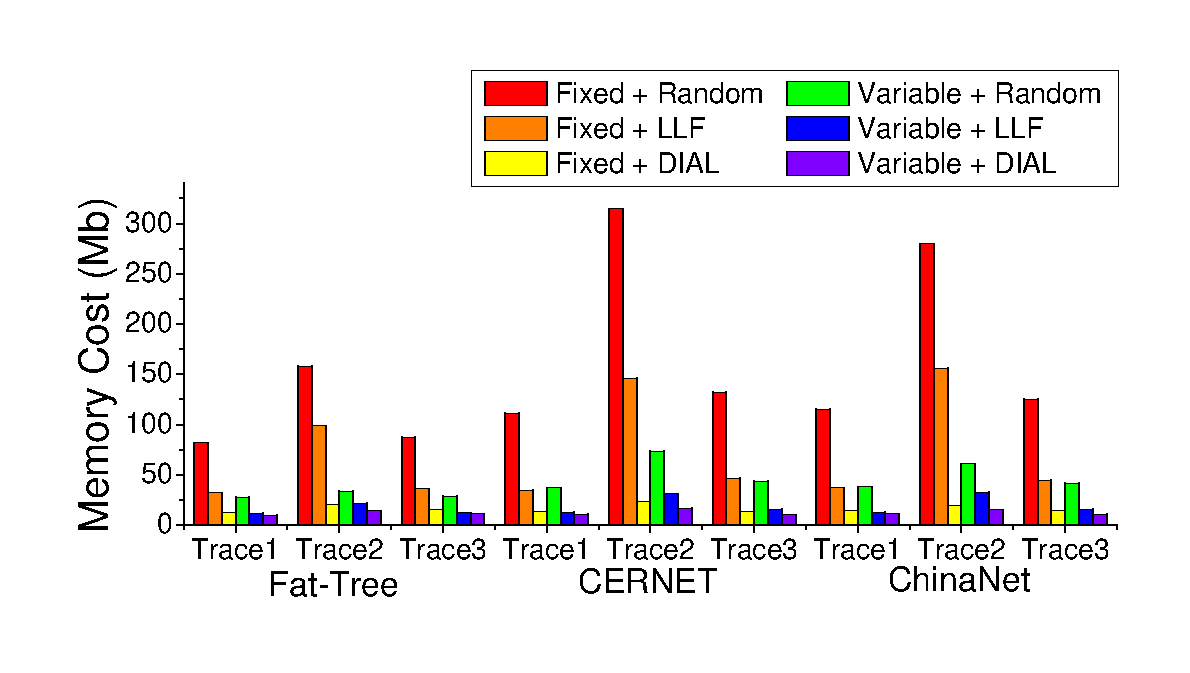
\includegraphics[width=0.5\textwidth]{DATA/cost.pdf}
\vspace{-0.4in}
\caption{Memory cost}
\label{fig:memory-cost}
\vspace{-0.2in}
\end{figure}

\begin{figure}[t]
\centering
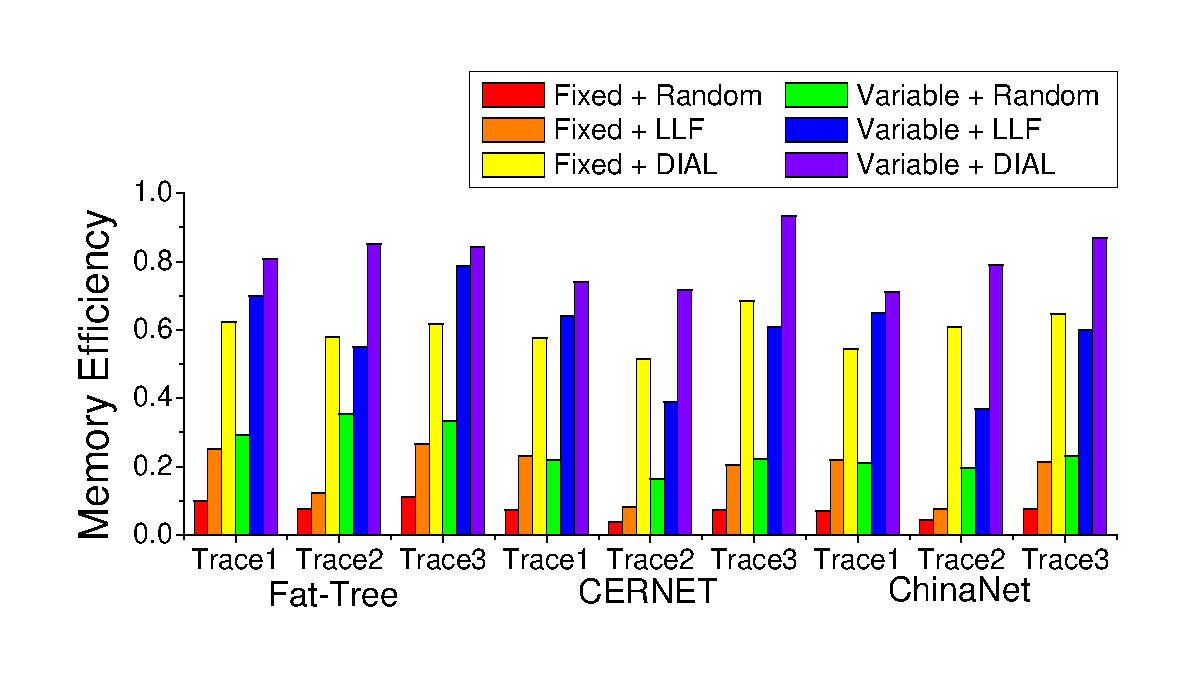
\includegraphics[width=0.5\textwidth]{DATA/efficiency.pdf}
\vspace{-0.4in}
\caption{Memory efficiency}
\label{fig:memory-efficiency}
\vspace{-0.2in}
\end{figure}

We further measure the overhead of extra Packet\_in messages when handling exceeding exceptions, as is denoted in the ``Costs'' field in Table~\ref{tab:result}.
We find that the ``Costs'' count is at the same order of magnitude with the flow count.
We know that in periodic network measurement in SDN, one flow has to lead the switch to communicate with the controller at least once when submitting the result at the end of the measurement period.
In DIAL, the extra message cost is introduced, which leads to an increase in the number of the same messages \eg, Packet\_in costs in OpenFlow, but that is still at the same order of magnitude, so we consider that it is endurable with high bandwidth SDN link. For example, the system in~\cite{Liu2017} has the 1Gbps SDN link.

\begin{table}[t]\small
 \caption{Some results of DIAL}
  \label{tab:result}
  \centering
  \begin{tabular}{ccccc}
    \toprule
    Topology & Trace  & \#Flow & T. O.  & Costs\\
    \midrule
    Fat-Tree & Trace1 & 0.9M   & 8.08Mb & 2.0M \\
    Fat-Tree & Trace2 & 1.5M  & 12.0Mb & 3.5M \\
    Fat-Tree & Trace3 & 1.0M  & 9.61Mb & 2.7M \\
    CERNET   & Trace1 & 0.9M   & 8.08Mb & 1.9M \\
    CERNET   & Trace2 & 1.5M  & 12.0Mb & 3.4M \\
    CERNET   & Trace3 & 1.0M  & 9.61Mb & 2.2M \\
    ChinaNet & Trace1 & 0.9M   & 8.08Mb & 1.9M \\
    ChinaNet & Trace2 & 1.5M  & 12.0Mb & 3.2M \\
    ChinaNet & Trace3 & 1.0M  & 9.61Mb & 2.3M \\
    \bottomrule
  \end{tabular}
  \vspace{-2ex}
\end{table}
